\section{Mixed meshfree formulation for modified Hellinger-Reissner weak form}\label{mixed}
\subsection{Reproducing kernel approximation for displacement}
This study approximates the displacement by adopting reproducing kernel approximation. As shown in Fig. \ref{fig2}, the mid-surface of the shell $\Omega$ is discretized by a set of meshfree nodes $\{\boldsymbol \xi_I\}_{I=1}^{n_p}$ in parametric configuration, where $n_p$ is the total number of meshfree nodes. The approximated displacement namely $\boldsymbol v^h$ can be expressed as:
\begin{equation}\label{approxv}
\boldsymbol v(\boldsymbol \xi) = \sum_{I=1}^{n_p} \Psi_I(\boldsymbol \xi) \boldsymbol d_I
\end{equation}
in which $\Psi_I$ and $\boldsymbol d_I$ is the shape function and nodal coefficient tensor related by node $\boldsymbol \xi_I$. According to reproducing kernel approximation \cite{liu1995}, the shape function takes the following form:
\begin{equation}
\Psi_I(\boldsymbol \xi) = \boldsymbol p^T(\boldsymbol \xi) \boldsymbol c(\boldsymbol \xi) \phi(\boldsymbol \xi_I - \boldsymbol \xi)
\end{equation}
where $\boldsymbol p$ is the basis function vector represented using the following quadratic function as:
\begin{equation}
        \boldsymbol p = \{1,\;\xi^1,\;\xi^2,\;(\xi^1)^2,\xi^1\xi^2,(\xi^2)^2\}^T
\end{equation}

The kernel function denoted by $\phi$ controls the support and smoothness of meshfree shape functions. The quintic B-spline function with square support is used herein as the kernel function:
\begin{equation}
\phi(\boldsymbol \xi_I - \boldsymbol \xi) = \phi(\hat s_1)\phi(\hat s_2), \quad \hat s_\alpha = \frac{\vert \xi^\alpha_I - \xi^\alpha\vert}{s_{\alpha I}}
\end{equation}
with
\begin{equation}
\phi(\hat s_\alpha) = \frac{1}{5!}\begin{cases}
(3-3\hat s_\alpha)^5 - 6(2-3\hat s_\alpha)^5 + 15(1-3\hat s_\alpha)^5 & \hat s_\alpha \le \frac{1}{3} \\
(3-3\hat s_\alpha)^5 - 6(2-3\hat s_\alpha)^5 & \frac{1}{3}<\hat s_\alpha \le \frac{2}{3} \\
(3-3\hat s_\alpha)^5 & \frac{2}{3}<\hat s_\alpha \le 1 \\
0 & \hat s_\alpha >1
\end{cases}
\end{equation}
and $s_{\alpha I}$ means the support size of meshfree shape function $\Psi_I$.

The unknown vector $\boldsymbol c$ in shape function are determined by the fulfillment of the so-called consistency condition:
\begin{equation}
\sum_{I=1}^{n_p} \Psi_I(\boldsymbol \xi)\boldsymbol p(\boldsymbol \xi_I) = \boldsymbol p(\boldsymbol \xi)
\end{equation}
or equivalently
\begin{equation}\label{cc}
\sum_{I=1}^{n_p} \Psi_I(\boldsymbol \xi)\boldsymbol p(\boldsymbol \xi_I-\boldsymbol \xi) = \boldsymbol p(\boldsymbol 0)
\end{equation}
Substituting Eq. (\ref{approxv}) into (\ref{cc}), yields:
\begin{equation}\label{A}
\boldsymbol A(\boldsymbol \xi) \boldsymbol c(\boldsymbol \xi) = \boldsymbol p(\boldsymbol 0)\quad \Rightarrow \quad
\boldsymbol c(\boldsymbol \xi) = \boldsymbol A^{-1}(\boldsymbol \xi)\boldsymbol p(\boldsymbol 0)
\end{equation}
where $\boldsymbol A$ is the moment matrix:
\begin{equation}
\boldsymbol A(\boldsymbol \xi) = \sum_{I=1}^{n_p}\phi(\boldsymbol \xi_I - \boldsymbol \xi) \boldsymbol p(\boldsymbol \xi_I-\boldsymbol \xi)\boldsymbol p^T(\boldsymbol \xi_I - \boldsymbol \xi)
\end{equation}
Substituting Eq. (\ref{A}) back into Eq. (\ref{approxv}), the expression of meshfree shape function can be written as:
\begin{equation}
\Psi_I(\boldsymbol \xi) = \boldsymbol p^T(\boldsymbol \xi_I - \boldsymbol \xi)\boldsymbol A^{-1}(\boldsymbol \xi) \boldsymbol p(\boldsymbol 0) \phi(\boldsymbol \xi_I-\boldsymbol \xi)
\end{equation}
\subsection{Reproducing kernel gradient smoothing approximation for effective stress and strain}
In Galerkin meshfree formulation, the mid-plane of thin shell $\Omega$ is split by a set of integration cells $\Omega_C$'s, $\cup_{C=1}^{n_e}\Omega_C\approx \Omega$, as shown in Fig. \ref{fig2}. With the inspiration of reproducing kernel smoothing framework, the Cartesian and covariant derivatives of displacement, $\boldsymbol v_{,\alpha}$ and $-\boldsymbol v_{,\alpha}\vert_\beta$, in strains $\varepsilon_{\alpha\beta}$, $\kappa_{\alpha\beta}$ are approximated by $(p-1)$-th order polynomials in each integration cells. In integration cell $\Omega_C$, the approximated derivatives and strains denoted by $\boldsymbol v^h_{,\alpha}$, $\varepsilon^h_{\alpha\beta}$ and $-\boldsymbol v^h_{,\alpha}\vert_\beta$, $\kappa^h_{\alpha\beta}$ can be expressed by:
\begin{equation}\label{approxsn1}
    \boldsymbol v^h_{,\alpha}(\boldsymbol \xi) = \boldsymbol q^T(\boldsymbol \xi) \boldsymbol d_{\alpha}^\varepsilon, \quad
    \varepsilon^h_{\alpha\beta}(\boldsymbol \xi) = \boldsymbol q^T(\boldsymbol \xi) \frac{1}{2}(\boldsymbol a_\alpha \cdot \boldsymbol d_{\beta}^\varepsilon + \boldsymbol a_\beta \cdot \boldsymbol d_{\alpha}^\varepsilon)
\end{equation}
\begin{equation}\label{approxsn2}
    -\boldsymbol v^h_{,\alpha}\vert_\beta(\boldsymbol \xi) = \boldsymbol q^T(\boldsymbol \xi) \boldsymbol d_{\alpha\beta}^\kappa , \quad
    \kappa^h_{\alpha\beta}(\boldsymbol \xi) = \boldsymbol q^T(\boldsymbol \xi) \boldsymbol a_3 \cdot \boldsymbol d_{\alpha\beta}^\kappa
\end{equation}
where $\boldsymbol q$ is the linear polynomial vector and has the following form:
\begin{equation}
\boldsymbol q = \{ 1,\; \xi^1,\; \xi^2\}^T
\end{equation}
and the $\boldsymbol d^\varepsilon_{\alpha}$, $\boldsymbol d^\kappa_{\alpha\beta}$ are the corresponding coefficient vector tensors. For the conciseness, the mixed usage of tensor and vector is introduced in this study. For instance, the component of coefficient tensor vector $\boldsymbol d^\varepsilon_{\alpha I}$, $\boldsymbol d^\varepsilon_\alpha = \{\boldsymbol d^\varepsilon_{\alpha I}\}$, is a three dimensional tensor, $\dim \boldsymbol d^\varepsilon_{\alpha I} = \dim \boldsymbol v$.

\begin{figure}[!ht]
\centering
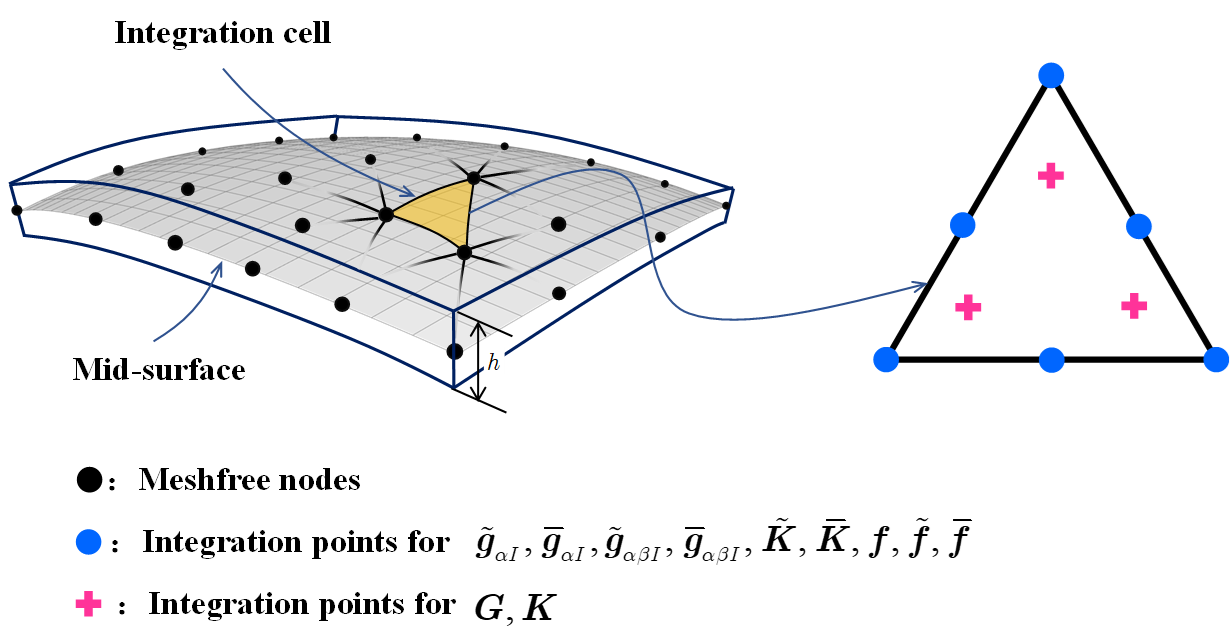
\includegraphics[width=\textwidth]{figures/2}
\caption{Integration scheme for Hu-Washizu weak form.}\label{fig2}
\end{figure}

To satisfy the integration constraint of thin shell problem, the approximated stresses $N^{\alpha\beta h}$, $M^{\alpha\beta h}$ were assumed to have a comparable form to strains, and yields:
\begin{equation}\label{approxse1}
N^{\alpha\beta h}(\boldsymbol \xi) = \boldsymbol q^T(\boldsymbol \xi) \boldsymbol a^\alpha \cdot \boldsymbol d^{\beta}_N,\quad
\boldsymbol a_\alpha N^{\alpha\beta h}(\boldsymbol \xi) = \boldsymbol q^T(\boldsymbol \xi) \boldsymbol d_N^\beta
\end{equation}
\begin{equation}\label{approxse2}
    M^{\alpha\beta h}(\boldsymbol \xi) = \boldsymbol q^T(\boldsymbol \xi) \boldsymbol a_3 \cdot \boldsymbol d^{\alpha\beta}_M,\quad
    \boldsymbol a_3 M^{\alpha\beta h}(\boldsymbol \xi) = \boldsymbol q^T(\boldsymbol \xi) \boldsymbol d^{\alpha\beta}_M
\end{equation}
substituting the approximations of Eqs. (\ref{approxv}), (\ref{approxsn1}), (\ref{approxsn2}), (\ref{approxse1}), (\ref{approxse2}) into Eqs. (\ref{w3}), (\ref{w4}) can express $\boldsymbol d^\varepsilon_\beta$ and $\boldsymbol d^\kappa_{\alpha\beta}$ by $\boldsymbol d$ as:
\begin{equation}\label{depsilon}
\boldsymbol d^\varepsilon_\beta = \boldsymbol G^{-1} \left (\sum_{I=1}^{n_p}(\tilde{\boldsymbol g}_{\beta I} - \bar{\boldsymbol g}_{\beta I}) \boldsymbol d_I + \hat{\boldsymbol g}_\beta \right )
\end{equation}
\begin{equation}\label{dkappa}
\boldsymbol d^\kappa_{\alpha\beta} = \boldsymbol G^{-1} \left (\sum_{I=1}^{n_p}(\tilde{\boldsymbol g}_{\alpha\beta I} - \bar{\boldsymbol g}_{\alpha\beta I})\boldsymbol d_I + \hat{\boldsymbol g}_{\alpha\beta} \right )
\end{equation}
with
\begin{equation}
\boldsymbol G = \int_{\Omega_C} \boldsymbol q^T \boldsymbol q d\Omega
\end{equation}
\begin{subequations}\label{gn}
\begin{align}
\tilde{\boldsymbol g}_{\beta I} &= \int_{\Gamma_C} \Psi_I \boldsymbol q n_\beta d\Gamma
- \int_{\Omega_C} \Psi_I \boldsymbol q_{\vert \beta} d\Omega \\
\bar{\boldsymbol g}_{\beta I} &= \int_{\Gamma_C\cap\Gamma_v} \Psi_I \boldsymbol q n_\beta d\Gamma \\
\hat{\boldsymbol g}_{\beta} &= \int_{\Gamma_C\cap\Gamma_v} \boldsymbol q n_\beta \bar{\boldsymbol v} d\Gamma 
\end{align}
\end{subequations}
\begin{subequations}\label{gm}
\begin{align}
\small
\begin{split}
\tilde{\boldsymbol g}_{\alpha\beta I} &= \int_{\Gamma_C} \Psi_{I,\gamma}n^\gamma \boldsymbol q n_\alpha n_\beta d\Gamma 
- \int_{\Gamma_C} \Psi_I(\boldsymbol q_{\vert \beta} n_\alpha + (\boldsymbol q s_\alpha n_\beta)_{,\gamma}s^\gamma) d\Gamma \\
&+ [[\Psi_I \boldsymbol q s_\alpha n_\beta]]_{\boldsymbol x\in C_C}
- \int_{\Omega_C} \Psi \boldsymbol q_{,\alpha\vert \beta} d\Omega \\
\end{split} \\
\small
\begin{split}
\bar{\boldsymbol g}_{\alpha\beta I} &= \int_{\Gamma_C\cap\Gamma_\theta} \Psi_{I,\gamma}n^\gamma \boldsymbol q n_\alpha n_\beta d\Gamma 
- \int_{\Gamma_C\cap\Gamma_v} \Psi_I(\boldsymbol q_{\vert \beta} n_\alpha + (\boldsymbol q s_\alpha n_\beta)_{,\gamma}s^\gamma) d\Gamma \\
&+ [[\Psi_I \boldsymbol q s_\alpha n_\beta]]_{\boldsymbol x\in C_C\cap C_v}
\end{split} \\
\small
\begin{split}
\hat{\boldsymbol g}_{\alpha\beta} &= \int_{\Gamma_C\cap\Gamma_\theta} \boldsymbol q n_\alpha n_\beta \boldsymbol a_3 \bar{\theta}_{\boldsymbol n} d\Gamma 
- \int_{\Gamma_C\cap\Gamma_v}(\boldsymbol q_{\vert \beta} n_\alpha + (\boldsymbol q s_\alpha n_\beta)_{,\gamma}s^\gamma)\bar{\boldsymbol v} d\Gamma \\
&+ [[\boldsymbol q s_\alpha n_\beta \bar{\boldsymbol v}]]_{\boldsymbol x\in C_C\cap C_v}
\end{split}
\end{align}
\end{subequations}
where the derivations of $\boldsymbol q_{\vert \beta}$, $\boldsymbol q_{,\alpha\vert\beta}$ are discussed in detail in \ref{derivative}. Further plugging Eqs. (\ref{depsilon}) and (\ref{dkappa}) back into Eqs. (\ref{approxsn1}) and (\ref{approxsn2}), respectively gives the final expression of $\boldsymbol v^h_{,\alpha}$, $\varepsilon^h_{\alpha\beta}$ and $-\boldsymbol v^h_{,\alpha\beta}$, $\boldsymbol \kappa^h_{\alpha\beta}$ as: \begin{subequations}
\begin{equation}
\boldsymbol v^h_{,\alpha} = \sum_{I=1}^{n_p}(
\tilde \Psi_{I,\alpha} - \bar \Psi_{I,\alpha}) \boldsymbol d_I +
\boldsymbol q^T \boldsymbol G^{-1}\hat{\boldsymbol g}_{\alpha}
\end{equation}
\begin{equation}\label{epsilonh}
\begin{split}
\varepsilon^h_{\alpha\beta} &= 
\sum_{I=1}^{n_p} \frac{1}{2}(\boldsymbol a_\alpha \tilde \Psi_{I,\beta} + \boldsymbol a_\beta \tilde \Psi_{I,\alpha}) \cdot \boldsymbol d_I 
- \sum_{I=1}^{n_p} \frac{1}{2}(\boldsymbol a_\alpha \bar \Psi_{I,\beta} + \boldsymbol a_\beta \bar \Psi_{I,\alpha}) \cdot \boldsymbol d_I \\
&+ \boldsymbol q^T \boldsymbol G^{-1} \frac{1}{2}(\boldsymbol a_\alpha \cdot \hat{\boldsymbol g}_{\beta} + \boldsymbol a_\beta \cdot \hat{\boldsymbol g}_{\alpha}) \\
&= \tilde \varepsilon^h_{\alpha\beta} - \bar \varepsilon^h_{\alpha\beta} + \hat \varepsilon^h_{\alpha\beta}
\end{split}
\end{equation}
\end{subequations}
\begin{subequations}
\begin{equation}
-\boldsymbol v^h_{,\alpha}\vert_\beta = \sum_{I=1}^{n_p} (
\tilde \Psi_{I,\alpha\beta} -
\bar \Psi_{I,\alpha\beta} ) \boldsymbol d_I +
\boldsymbol q^T \boldsymbol G^{-1}\hat{\boldsymbol g}_{\alpha\beta}
\end{equation}
\begin{equation}\label{kappah}
\begin{split}
\kappa^h_{\alpha\beta} &= \sum_{I=1}^{n_p} \tilde \Psi_{I,\alpha\beta} \boldsymbol a_3 \cdot \boldsymbol d_I
- \sum_{I=1}^{n_p} \bar \Psi_{I,\alpha\beta} \boldsymbol a_3 \cdot \boldsymbol d_I +
\boldsymbol q^T \boldsymbol G^{-1}\boldsymbol a_3 \cdot \hat{\boldsymbol g}_{\alpha\beta} \\
&= \tilde \kappa^h_{\alpha\beta} - \bar \kappa^h_{\alpha\beta} + \hat \kappa^h_{\alpha\beta}
\end{split}
\end{equation}
\end{subequations}
with
\begin{equation}\label{epsilon2}
\left \{
\begin{split}
\tilde \varepsilon^h_{\alpha\beta} &= \sum_{I=1}^{n_p} \frac{1}{2}(\boldsymbol a_\alpha \tilde \Psi_{I,\beta} + \boldsymbol a_\beta \tilde \Psi_{I,\alpha}) \cdot \boldsymbol d_I
=\sum_{I=1}^{n_p} \tilde{\boldsymbol \varepsilon}_{\alpha\beta I} \cdot \boldsymbol d_I \\
\bar \varepsilon^h_{\alpha\beta} &= \sum_{I=1}^{n_p} \frac{1}{2}(\boldsymbol a_\alpha \bar \Psi_{I,\beta} + \boldsymbol a_\beta \bar \Psi_{I,\alpha}) \cdot \boldsymbol d_I
=\sum_{I=1}^{n_p} \bar{\boldsymbol \varepsilon}_{\alpha\beta I} \cdot \boldsymbol d_I \\
\hat \varepsilon^h_{\alpha\beta} &= \boldsymbol q^T \boldsymbol G^{-1} \frac{1}{2}(\boldsymbol a_\alpha\cdot\hat{\boldsymbol g}_\beta + \boldsymbol a_\beta \cdot \hat{\boldsymbol g}_\alpha)
\end{split}
\right .
\end{equation}
\begin{equation}
\left \{
\begin{split}
&\tilde{\Psi}_{I,\alpha}(\boldsymbol \xi) = \boldsymbol q^T(\boldsymbol \xi) \boldsymbol G^{-1} \tilde{\boldsymbol g}_{\alpha I} \\
&\bar{\Psi}_{I,\alpha}(\boldsymbol \xi) = \boldsymbol q^T(\boldsymbol \xi) \boldsymbol G^{-1} \bar{\boldsymbol g}_{\alpha I} \\
&\tilde{\boldsymbol \varepsilon}_{\alpha\beta I} = \frac{1}{2}(\boldsymbol a_\alpha \tilde \Psi_{I,\beta} + \boldsymbol a_\beta \tilde \Psi_{I,\alpha}) \\
&\bar{\boldsymbol \varepsilon}_{\alpha\beta I} = \frac{1}{2}(\boldsymbol a_\alpha \bar \Psi_{I,\beta} + \boldsymbol a_\beta \bar \Psi_{I,\alpha})
\end{split}
\right .
\end{equation}
\begin{equation}\label{kappa2}
\left \{
\begin{split}
\tilde \kappa^h_{\alpha\beta} &= \sum_{I=1}^{n_p} \tilde \Psi_{I,\alpha\beta}\boldsymbol a_3 \cdot \boldsymbol d_I 
= \sum_{I = 1}^{n_p} \tilde{\boldsymbol \kappa}_{\alpha\beta I} \cdot \boldsymbol d_I\\
\bar \kappa^h_{\alpha\beta} &= \sum_{I=1}^{n_p} \bar \Psi_{I,\alpha\beta}\boldsymbol a_3 \cdot \boldsymbol d_I
= \sum_{I = 1}^{n_p} \bar{\boldsymbol \kappa}_{\alpha\beta I} \cdot \boldsymbol d_I \\
\hat \kappa^h_{\alpha\beta} &= \boldsymbol q^T \boldsymbol G^{-1} \boldsymbol a_3 \cdot \hat{\boldsymbol g}_{\alpha\beta}
\end{split}
\right .
\end{equation}
\begin{equation}
\left \{
\begin{split}
&\tilde{\Psi}_{I,\alpha\beta}(\boldsymbol \xi) = \boldsymbol q^T(\boldsymbol \xi) \boldsymbol G^{-1} \tilde{\boldsymbol g}_{\alpha\beta I} \\
&\bar{\Psi}_{I,\alpha\beta}(\boldsymbol \xi) = \boldsymbol q^T(\boldsymbol \xi) \boldsymbol G^{-1} \tilde{\boldsymbol g}_{\alpha\beta I} \\
&\tilde{\boldsymbol \kappa}_{\alpha\beta I} = \tilde \Psi_{I,\alpha\beta}\boldsymbol a_3 \\
&\bar {\boldsymbol \kappa}_{\alpha\beta I} = \bar \Psi_{I,\alpha\beta}\boldsymbol a_3 \\
\end{split}
\right .
\end{equation}

% Furthermore, taking Eqs. (\ref{approxsn1}) and (\ref{approxsn2}) into Eqs.(\ref{w1}) and (\ref{w2}) can obtain the approximated effective stresses $N^{\alpha\beta h}$, $M^{\alpha\beta h}$ and their coefficients $\boldsymbol d_N^\beta$, $\boldsymbol d_M^{\alpha\beta}$ as:
% \begin{equation}\label{d_N1}
%  \delta \boldsymbol d^\varepsilon_\alpha \cdot \boldsymbol G^{\alpha\eta}_N \cdot \boldsymbol d^\varepsilon_\eta = \delta \boldsymbol d^\varepsilon_\alpha \cdot \boldsymbol d_N^\alpha \boldsymbol G \quad\Rightarrow \quad & \boldsymbol d_N^\alpha = \boldsymbol G^{-1} \boldsymbol G_N^{\alpha\eta} \cdot \boldsymbol d^\varepsilon_\eta
% \end{equation}
% \begin{equation}\label{d_M1}
%  \delta \boldsymbol d^\kappa_{\alpha\beta} : \boldsymbol G_M^{\alpha\beta\gamma\eta} : \boldsymbol d^\kappa_{\gamma\eta} \boldsymbol G = \delta \boldsymbol d^\kappa_{\alpha\beta} \cdot \boldsymbol d_M^{\alpha\beta} \boldsymbol G \\
% \Rightarrow \; \boldsymbol d_M^{\alpha\beta} = \boldsymbol G^{-1} \boldsymbol G_{\alpha\beta}^M \cdot \boldsymbol d^\kappa_{\gamma\eta}
% \end{equation}
% with
% \begin{equation}
% \boldsymbol G^{\alpha\eta}_N = \int_{\Omega_C} \boldsymbol a_\beta hC^{\alpha\beta\gamma\eta} \boldsymbol a_\gamma \boldsymbol q \boldsymbol q^T d\Omega
% \end{equation}
% \begin{equation}
% \boldsymbol G^{\alpha\beta\gamma\eta}_M = \int_{\Omega_C} \boldsymbol a_3 \frac{h^3}{12}C^{\alpha\beta\gamma\eta}\boldsymbol a_3 \boldsymbol q\boldsymbol q^T d\Omega
% \end{equation}
%  
% Finally, taking Eqs. (\ref{d_N1}) and (\ref{d_M1}) back to Eqs. (\ref{approxse1}), (\ref{approxse2}) can express the components of stresses as follows:
% \begin{equation}\label{Nh}
% N^{\alpha\beta h} = \boldsymbol q^T \boldsymbol G^{-1}\frac{1}{2}(\boldsymbol a^\alpha \cdot \boldsymbol G^{\beta\gamma}_{N} + \boldsymbol a^\beta \cdot \boldsymbol G^{\alpha\gamma}_N) \cdot \boldsymbol d^{\varepsilon}_\gamma
% \end{equation}
% \begin{equation}\label{Mh}
% M^{\alpha\beta h} = \boldsymbol q^T \boldsymbol G^{-1} \boldsymbol a_3 \cdot \boldsymbol G^{\alpha\beta\gamma\eta}_M \cdot \boldsymbol d^\kappa_{\gamma\eta}
% \end{equation}

It has to be noted that, referring to reproducing kernel gradient smoothing framework \cite{wang2019a}, $\tilde \Psi_{I,\alpha}$, $\tilde \Psi_{I,\alpha\beta}$ are actually the first and second order smoothed gradients in curvilinear coordinates.If the right hand side integration constraints for first and second order gradients are $\tilde{\boldsymbol g}_{\alpha I}$ and $\tilde{\boldsymbol g}_{\alpha \beta I}$, respectively, then this formulation can satisfy  the variational consistency for the second order polynomials. It should be mentioned that in curved model, the variational consistency for non-polynomial functions, such as trigonometric functions, should be required for the polynomial solution. Even with high order polynomial variational consistency, the proposed formulation cannot exactly reproduce the solution spanned by the basis functions. However, the accuracy of reproducing kernel smoothed gradients is still superior than the traditional meshfree formulation. The numerical examples in the following section will better demonstrate to the precision of the reproducing kernel smoothed gradients.

